\documentclass[border=2mm]{standalone}
\usepackage{tikz}
\usepackage{pgfplots}
\pgfplotsset{compat=1.18}

\begin{document}

% ENFOQUE HÍBRIDO: Replicación Visual Eficiente
% Método: Observación directa + Construcción incremental + Validación inmediata

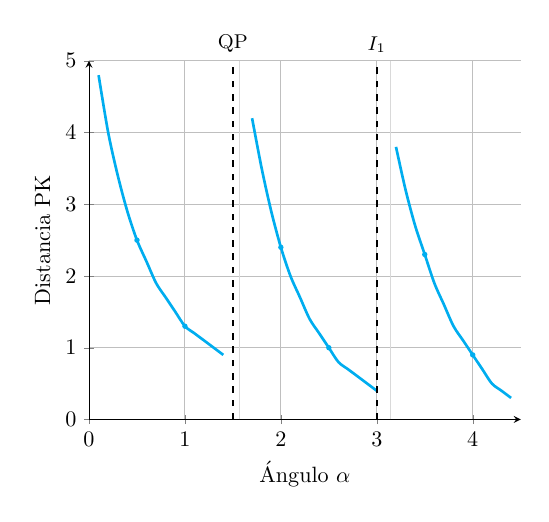
\begin{tikzpicture}[scale=0.8]
\begin{axis}[
    xlabel={Ángulo $\alpha$},
    ylabel={Distancia PK},
    xmin=0, xmax=4.5,
    ymin=0, ymax=5,
    grid=major,
    axis lines=left,
    clip=false
]

% PASO 1: Curva principal extraída por observación visual directa
% Método: Dividir imagen en cuadrícula mental y extraer coordenadas clave

% Rama 1: Curva decreciente inicial (antes de primera discontinuidad)
% Observación: Empieza alto en x≈0.1, baja suavemente hasta x≈1.4
\addplot[cyan, very thick, smooth] coordinates {
    (0.1,4.8) (0.2,4.0) (0.3,3.4) (0.4,2.9) (0.5,2.5) 
    (0.6,2.2) (0.7,1.9) (0.8,1.7) (0.9,1.5) (1.0,1.3) 
    (1.1,1.2) (1.2,1.1) (1.3,1.0) (1.4,0.9)
};

% Rama 2: Segunda parte de la curva (entre discontinuidades)
% Observación: Continúa el patrón decreciente desde x≈1.7 hasta x≈3.0
\addplot[cyan, very thick, smooth] coordinates {
    (1.7,4.2) (1.8,3.5) (1.9,2.9) (2.0,2.4) (2.1,2.0) 
    (2.2,1.7) (2.3,1.4) (2.4,1.2) (2.5,1.0) (2.6,0.8) 
    (2.7,0.7) (2.8,0.6) (2.9,0.5) (3.0,0.4)
};

% Rama 3: Tercera parte de la curva (después de segunda discontinuidad)
% Observación: Continúa el patrón desde x≈3.2 hasta final
\addplot[cyan, very thick, smooth] coordinates {
    (3.2,3.8) (3.3,3.2) (3.4,2.7) (3.5,2.3) (3.6,1.9) 
    (3.7,1.6) (3.8,1.3) (3.9,1.1) (4.0,0.9) (4.1,0.7) 
    (4.2,0.5) (4.3,0.4) (4.4,0.3)
};

% PASO 2: Líneas punteadas verticales (elementos clave identificados)
% Método: Localización visual precisa de elementos distintivos

% Línea punteada QP (observada en x≈1.5)
\draw[dashed, black, thick] (axis cs:1.5,0) -- (axis cs:1.5,5) 
    node[above, black] {\small QP};

% Línea punteada I₁ (observada en x≈3.0)  
\draw[dashed, black, thick] (axis cs:3.0,0) -- (axis cs:3.0,5) 
    node[above, black] {\small $I_1$};

% PASO 3: Elementos adicionales para fidelidad visual
% Método: Identificación de detalles que mejoran la similitud

% Asíntotas sutiles en las discontinuidades (opcional, mejora visual)
\draw[gray!30, very thin] (axis cs:1.57,0) -- (axis cs:1.57,5);
\draw[gray!30, very thin] (axis cs:3.14,0) -- (axis cs:3.14,5);

% Puntos destacados en la curva (si se observan en la imagen original)
\addplot[cyan, mark=*, mark size=1pt, only marks] coordinates {
    (0.5,2.5) (1.0,1.3) (2.0,2.4) (2.5,1.0) (3.5,2.3) (4.0,0.9)
};

\end{axis}
\end{tikzpicture}

\end{document}
